\subsection{连通与分隔}
\label{sec:graph-connectivity-separation}

第~\ref{sec:graph-adjacency-paths}小节的可达关系一次只回答两个顶点之间的问题。道路网规划还需要整体的回答：全部城市分成几片互相到达的区域，封闭哪些路口或道路会把区域切开。前一个问题由可达关系的等价类回答，有向图中则要区分强、弱两种连通；后一个问题要看删除顶点或边以后是否还有替代路径。

\subsubsection{无向图的连通分量}
\label{sec:graph-conn-components}

我们想把全部城市分成若干片，同一片中的城市两两可以互相到达，不同片之间无路可通；有了这样的划分，“能否互相到达”就只需看是否在同一片中。第~\ref{sec:graph-conn-reachability}小节说明，无向图中的可达关系是等价关系；等价类两两不交、并起来恰为$V$，所以它们恰好构成这样的划分。

\begin{definition}[连通分量]
\label{def:graph-conn-component}
无向图$\mathcal G=(V,E)$中可达关系的每个等价类$C\subseteq V$称为$\mathcal G$的一个\term{连通分量}（connected component）；有时也把诱导子图$\mathcal G[C]$称为连通分量。若$\mathcal G$非空且恰有一个连通分量，即任意两个顶点之间都有路径，就称$\mathcal G$是\term{连通}（connected）的。
\end{definition}

这个划分有三条直接的性质。连接同一分量中两点的路径不会离开该分量，因为路径上的每个顶点都与起点可达，所以$\mathcal G[C]$本身连通。不同分量之间没有边，否则两端可达，应属同一分量。划分只取决于可达关系，由图唯一确定。

图~\ref{fig:graph-conn-components}(a)是三角形$\{1,2,3\}$加上孤立顶点$4$，有两个分量$\{1,2,3\}$与$\{4\}$，不连通。空图的分量数为$0$，按定义不算连通，用“恰有一个分量”判断连通时要先排除这个情形。

\begin{figure*}[!htb]
  \centering
  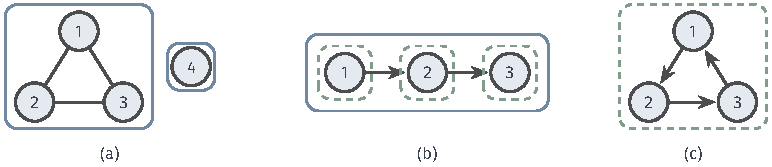
\includegraphics[width=130.652mm]{figures/01-basic-mathematics/04-graphs/tikz/c1-components/figure.pdf}
  \caption{连通分量。蓝色实线框是无向图或底层无向图的连通分量，绿色虚线框是强连通分量。(a)孤立点自成一个分量；(b)单向链$1\to2\to3$忽略方向后连成一片，但没有两个顶点能互相到达，每个顶点自成一个强分量；(c)有向环上任意两个顶点都能互相到达，三个顶点属于同一个强分量。}
  \label{fig:graph-conn-components}
\end{figure*}

\paragraph{分量划分的核对}
核对别人给出的划分不必逐对找路径，上面的前两条性质反过来就够了。

\begin{lemma}[分量划分的核对]
\label{lem:graph-conn-component-check}
设$C_1,\ldots,C_c$是无向图$\mathcal G$的顶点集的一个划分。若每个$\mathcal G[C_k]$都连通，并且没有一条边的两端位于不同的块中，则$C_1,\ldots,C_c$恰好是$\mathcal G$的全部连通分量。
\end{lemma}

\begin{proof}
同一块中的两点由块内连通而可达。反过来，若$j$从$i$可达，取一条行走，它的每一步沿一条边，而没有边跨越不同的块，所以$i,j$在同一块中。于是各块就是可达关系的等价类。
\end{proof}

于是核对分两步：给顶点写上块编号，逐条扫描边，检查两端编号相同；再对每一块给出把块内顶点连在一起的边。图~\ref{fig:graph-conn-components}(a)的划分$(1,1,1,2)$两步都通过；若把贯穿图划分为$\{1,2\}$与$\{3,4\}$，第一步就在边$\{1,3\}$处失败。

第二步所需的块内连接在第~\ref{sec:graph-trees-forests}小节整理为生成森林；从零求出全部分量，由第~\ref{sec:graph-connectivity-computation}节在与$n+m$成正比的时间内完成。

一张图是否连通，取决于删去连接以后有没有替代路径。在贯穿图中删除边$\{2,3\}$，$2$与$3$仍可经$1$或$4$相连；在图~\ref{fig:graph-conn-cut-bridge}(a)中删除连接两个三角形的边$\{3,4\}$，图就分成两个分量。两次都只删除一条边，结果不同是因为前者的边位于环上，环的另一侧提供了替代路径。第~\ref{sec:graph-conn-cut-bridge}小节会把这一观察写成桥的判别条件。

\subsubsection{强连通与弱连通}
\label{sec:graph-conn-strong-weak}

有向图中可达不是等价关系，不能直接用来划分顶点。修补的办法有两种：要求双向都可达，回答哪些顶点能“绕得回来”；或者忽略方向，只问是否连成一片。

若$j$从$i$可达且$i$从$j$可达，称$i,j$相互可达。相互可达关系是自反的（零长度行走）、对称的（定义对$i,j$对称）、传递的（两个方向分别首尾相接），因此是等价关系。它的等价类称为\term{强连通分量}（strongly connected component）；若有向图非空且只有一个强连通分量，就称它\term{强连通}（strongly connected）。

忽略方向的办法用底层无向图（第~\ref{sec:graph-conn-directions}小节）的连通分量划分顶点，所得的分量称为原图的\term{弱连通分量}（weakly connected component）；底层无向图连通时，称原有向图\term{弱连通}（weakly connected）。

在小图上可以直接读出两种分量。记$R^+(v)$与$R^-(v)$分别为从$v$可达与能到达$v$的顶点集（都含$v$），由定义，$v$所在的强分量是
\[
R^+(v)\cap R^-(v);
\]
弱分量则在底层无向图上读出。

图~\ref{fig:graph-conn-components}(b)的单向链中，$R^+(2)=\{2,3\}$，$R^-(2)=\{1,2\}$，所以$2$所在的强分量是
\[
R^+(2)\cap R^-(2)=\{2,3\}\cap\{1,2\}=\{2\}.
\]
同理三个顶点各成一个强分量，却只有一个弱分量。(c)的有向环中两个可达集都是$\{1,2,3\}$，图强连通。在大图上求全部强分量的线性时间方法见第~\ref{sec:graph-connectivity-computation}节。

有向路径去掉箭头后是底层无向图中的路径，所以每个强分量都包含在某个弱分量之内，强连通蕴含弱连通。单向链说明反过来不成立。需要回答“能否往返”时，必须使用强分量。

\subsubsection{分隔集}
\label{sec:graph-conn-separators}

规划者还关心脆弱性：封闭哪些路口能把两个区域隔开。被封闭的路口不能属于要隔开的两组本身；“隔开”的含义是，删掉这些路口以后，两组之间一条路径也不剩。

\begin{definition}[分隔]
\label{def:graph-conn-separation}
设$A,B,S\subseteq V$两两不相交。若在$\mathcal G-S$中不存在从$A$中顶点到$B$中顶点的路径，就称$S$\term{分隔}（separate）$A$与$B$，称$S$为$A$与$B$之间的一个\term{分隔集}（separator）。
\end{definition}

等价地，$\mathcal G$中从$A$到$B$的每条路径都至少经过$S$中的一个顶点，因为$\mathcal G-S$中的路径就是$\mathcal G$中避开$S$的路径。所以验证一个候选集要考虑全部路径，找到一条被阻断的路径并不够。

核对时却不必列举路径：在$\mathcal G-S$中从$A$出发求出可达集$R$（第~\ref{sec:graph-bfs}节的广度优先遍历允许以一组顶点为起点），$S$分隔$A$与$B$当且仅当$R\cap B=\varnothing$。若$A$与$B$原本位于不同分量，空集就分隔它们。

在图~\ref{fig:graph-conn-separator-sets}中取$A=\{1\}$、$B=\{4\}$。删除$\{2\}$后$R=\{1,3,4\}$，路径$(1,3,4)$仍在，$\{2\}$不是分隔集；删除$\{2,3\}$后$1$的邻居全被删去，$R=\{1\}$，$\{2,3\}$是分隔集。

\begin{figure}[!htb]
  \centering
  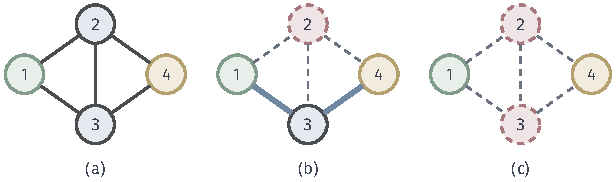
\includegraphics[width=104.186mm]{figures/01-basic-mathematics/04-graphs/tikz/c1-separator-sets/figure.pdf}
  \caption{在贯穿图中检验分隔集，$A=\{1\}$为绿色，$B=\{4\}$为黄色，被删除的候选集$S$为红色虚线顶点。(b)删除$\{2\}$后蓝色路径$(1,3,4)$仍然存在，$\{2\}$不是分隔集；(c)删除$\{2,3\}$后从$1$到$4$没有路径，$\{2,3\}$分隔$\{1\}$与$\{4\}$。}
  \label{fig:graph-conn-separator-sets}
\end{figure}

不指定两组顶点时，分隔集由删除后的分量给出。对连通图$\mathcal G$，若$\mathcal G-S$不连通，则$S$分隔$\mathcal G-S$中任意两个不同分量的顶点集。例如贯穿图删除$\{2,3\}$后余下$\{1\}$与$\{4\}$。第~\ref{sec:graph-separator-blocks}节将沿这样的分隔集把图分成可以分别处理的块。

\subsubsection{割点与桥}
\label{sec:graph-conn-cut-bridge}

最脆弱的情形是只失去一个路口或一条道路，网络就断开。删除顶点$v$后$\mathcal G-\{v\}$的分量数大于$\mathcal G$的分量数，称$v$为\term{割点}（cut vertex）；删除边$e$后$\mathcal G-e$的分量数大于$\mathcal G$的分量数，称$e$为\term{桥}（bridge）。

图~\ref{fig:graph-conn-cut-bridge}(a)由两个三角形$\{1,2,3\}$、$\{4,5,6\}$和边$\{3,4\}$组成，$3,4$是割点，$\{3,4\}$是桥，三角形内部的边和顶点$1,2,5,6$都不是；(b)的链中，中间顶点$2$是割点，两条边都是桥；(c)的三角形中，删除任意一个顶点或一条边都不会断开。

\begin{figure*}[!htb]
  \centering
  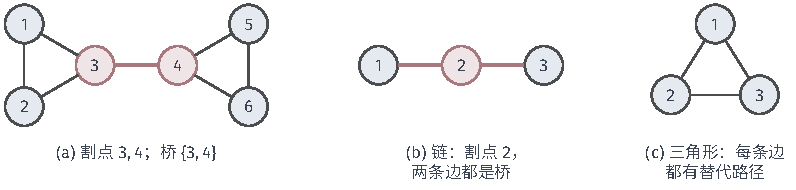
\includegraphics[width=132.687mm]{figures/01-basic-mathematics/04-graphs/tikz/c1-cut-vertex-bridge/figure.pdf}
  \caption{割点与桥，红色顶点为割点，红色粗边为桥。(a)两个三角形由一条边相连，这条边是桥，它的两个端点是割点；(b)链上每条边都是桥，中间顶点是割点，端点$1,3$虽是桥的端点却不是割点；(c)三角形的每条边都位于环上，删除任何一条边或一个顶点都不会断开。}
  \label{fig:graph-conn-cut-bridge}
\end{figure*}

\paragraph{桥的判别}
按定义判断桥要比较删除前后的分量数。下面的定理把它换成只看这条边两端的条件，并说明环正是替代路径的来源。

\begin{theorem}[桥的判别]
\label{thm:graph-conn-bridge-cycle}
设$e=\{i,j\}$是无向图$\mathcal G$的一条边。以下三条等价：(1)$e$是桥；(2)$\mathcal G-e$中没有从$i$到$j$的路径；(3)$e$不在$\mathcal G$的任何环上。并且删除任何一条边，分量数至多增加$1$。
\end{theorem}

\begin{proof}
删除$e$只可能拆开$e$所在的分量$C$。$C$中任一顶点$x$在原图中有到$i$的路径；若它经过$e$，取它第一次到达$i$或$j$之前的部分。这部分不含$e$，所以删除后$x$仍连到$i$或$j$。因此$\mathcal G-e$中$C$至多分成$i$所在和$j$所在两部分，分量数至多增加$1$，并且增加当且仅当$i,j$不再连通，即(1)与(2)等价。

若$e$在某个环上，环的另一侧就是$\mathcal G-e$中从$i$到$j$的路径，所以(2)蕴含(3)；反过来，$\mathcal G-e$中从$i$到$j$的路径长度至少为$2$，接上$e$就是一个环，所以(3)蕴含(2)。
\end{proof}

\paragraph{割点与桥的检验}
由定理，检验$e=\{i,j\}$是否为桥，只需在$\mathcal G-e$中从$i$做一次可达性搜索，看能否到达$j$。例如在图~\ref{fig:graph-conn-cut-bridge}(a)中，删去$\{3,4\}$后从$3$只能到达$\{1,2,3\}$，它是桥；删去$\{1,2\}$后仍可经$3$到达$2$，它不是桥。

检验顶点$v$是否为割点时，度为$0$或$1$的顶点可直接排除。其余情况下，删去$v$后从它的一个邻居出发，看能否到达它的其余全部邻居。只看邻居就够了：$v$所在分量中的其他顶点，沿通往$v$的路径走到第一次遇到$v$的邻居为止，这一段避开了$v$，所以它们在删去$v$后仍连到$v$的某个邻居。于是分量是否断开，只取决于$v$的邻居之间是否仍然连通。逐一检验全部顶点或全部边，每次都要做一次这样的搜索。

删点与删边的效果并不对称。删除一个顶点会同时删除它的全部邻边，可能把分量拆成很多块：星形图删除中心顶点后，其余每个顶点都自成一个分量；删除一条边却至多增加一个分量。桥的端点不一定是割点，例如图~\ref{fig:graph-conn-cut-bridge}(b)的端点$1$；没有桥的图也可能有割点，例如两个三角形共用一个顶点。所以“删点能否断开”与“删边能否断开”需要分别检查。

\subsection{团与独立集}
\label{sec:graph-cliques-independent-sets}

连通与分隔考察的是顶点之间能否经由一串边间接相连。若只看一步之内的直接邻接，一个顶点子集$S\subseteq V$内部还有两种相反的极端结构：一种是$S$中任意两个顶点都有边直接相连，代表彼此完全耦合或两两冲突的群体；另一种是$S$中任意两个顶点都没有边相连，代表彼此互不干扰、可以同时入选的对象集合。在社交网络或变量交互图中，有时要找出内部两两都有直接联系的一群顶点；而在选址或调度问题中，若把冲突关系画成边，又要选出内部两两都不冲突的一组顶点。

\begin{definition}[完全图、团与独立集]
\label{def:graph-clique-independent}
设$\mathcal G=(V,E)$是无向图。若$V$中任意两个不同顶点都相邻，即$|E|=\binom{|V|}{2}$，称$\mathcal G$为\term{完全图}（complete graph），有$n$个顶点的完全图记作$K_n$。

对顶点子集$S\subseteq V$：若$S$中任意两个不同顶点在$\mathcal G$中都相邻（即诱导子图$\mathcal G[S]$是完全图），称$S$为$\mathcal G$的一个\term{团}（clique）；若$S$中任意两个顶点在$\mathcal G$中都不相邻（即诱导子图$\mathcal G[S]$没有边），称$S$为$\mathcal G$的一个\term{独立集}（independent set），也称稳定集。
\end{definition}

单个顶点组成的集合既是团也是独立集。讨论团的大小时，需要区分“不能再往里添点”和“点数最多”两个层次：若团$S$不能通过加入$V\setminus S$中的任何顶点而扩大成更大的团，称$S$为\term{极大团}（maximal clique）；包含顶点数最多的团称为\term{最大团}（maximum clique），其顶点数称为$\mathcal G$的\term{团数}（clique number），记作$\omega(\mathcal G)$。同样，不能再添点的独立集称为极大独立集，包含顶点数最多的独立集称为最大独立集，其顶点数称为$\mathcal G$的\term{独立数}（independence number），记作$\alpha(\mathcal G)$。

团与独立集的条件正好把“有边”和“无边”对调。把一张图所有相邻的顶点对改成不相邻、不相邻的顶点对改成相邻，就得到它的补图。

\begin{definition}[补图]
\label{def:graph-complement}
设$\mathcal G=(V,E)$是简单无向图。以$V$为顶点集、以
\[
\overline E=\bigl\{\{u,v\}:u,v\in V,\,u\neq v,\,\{u,v\}\notin E\bigr\}
\]
为边集的无向图称为$\mathcal G$的\term{补图}（complement graph），记作$\overline{\mathcal G}=(V,\overline E)$。
\end{definition}

由定义立即可得团与独立集在补图运算下的对偶关系。

\begin{theorem}[团与独立集的补图对偶]
\label{thm:graph-clique-independent-complement}
设$\mathcal G=(V,E)$是简单无向图，$S\subseteq V$。$S$是$\mathcal G$的独立集，当且仅当$S$是补图$\overline{\mathcal G}$的团。特别地，
\begin{equation}
\alpha(\mathcal G)=\omega(\overline{\mathcal G}),\qquad
\omega(\mathcal G)=\alpha(\overline{\mathcal G}).
\label{eq:graph-clique-independent-complement}
\end{equation}
\end{theorem}

\begin{proof}
$S$是$\mathcal G$的独立集，当且仅当对任意$u,v\in S$（$u\neq v$）都有$\{u,v\}\notin E$；按补图的定义，这当且仅当对任意$u,v\in S$（$u\neq v$）都有$\{u,v\}\in\overline E$，即$S$是$\overline{\mathcal G}$的团。对所有满足条件的子集$S$取最大基数，即得$\alpha(\mathcal G)=\omega(\overline{\mathcal G})$；再注意到$\overline{\overline{\mathcal G}}=\mathcal G$，立得$\omega(\mathcal G)=\alpha(\overline{\mathcal G})$。
\end{proof}

在贯穿图\eqref{eq:graph-conn-running-graph}中，三角形$\{1,2,3\}$与$\{2,3,4\}$内部两两相邻，而全集$\{1,2,3,4\}$缺少边$\{1,4\}$，因此这两个三角形既是极大团也是最大团，$\omega(\mathcal G)=3$。至于独立集，由于$1$和$4$不相邻，$\{1,4\}$是最大独立集，$\alpha(\mathcal G)=2$；单点集$\{2\}$也是极大独立集（因为$2$与$1,3,4$全部相邻，无法再添任何顶点），但它只有$1$个顶点，不是最大独立集，可见“极大”不等于“最大”。转到补图$\overline{\mathcal G}$时，四点间原本缺少的唯一一条边$\{1,4\}$成了$\overline{\mathcal G}$中唯一的边（图~\ref{fig:graph-clique-indep-cover}(b)），此时$\{1,4\}$恰好是$\overline{\mathcal G}$的最大团（$\omega(\overline{\mathcal G})=2=\alpha(\mathcal G)$），而原图的最大团$\{1,2,3\}$在$\overline{\mathcal G}$中一条边也没有，成为最大独立集（$\alpha(\overline{\mathcal G})=3=\omega(\mathcal G)$）。若进一步把顶点集$V$划分为尽量少的若干个独立集，使相邻顶点分属不同块，就得到第~\ref{sec:graph-coloring}节的正常顶点着色问题。

\subsection{点覆盖与支配集}
\label{sec:graph-vertex-cover-dominating}

团与独立集关心的是所选子集$S$内部有没有边；另一类常见任务关心的是如何用尽量少的顶点去“管住”整张图。根据被管住的对象是图中的全部边还是全部顶点，这类任务分为点覆盖与支配集两种结构：前者要求每条边至少有一个端点入选，后者要求每个未入选顶点至少有一个邻居入选。

\subsubsection{点覆盖}
\label{sec:graph-vertex-cover}

如果把边看成需要监控的道路，在路口安装监控器，使得每一条道路至少有一端装有监控器，所选的路口集合就是一个点覆盖。

\begin{definition}[点覆盖]
\label{def:graph-vertex-cover}
设$\mathcal G=(V,E)$是无向图。若顶点子集$C\subseteq V$满足每条边$e=\{u,v\}\in E$都至少有一个端点在$C$中（即$e\cap C\neq\varnothing$），就称$C$为$\mathcal G$的一个\term{顶点覆盖}（vertex cover），简称点覆盖。包含顶点数最少的点覆盖称为最小点覆盖，其顶点数称为$\mathcal G$的\term{顶点覆盖数}（vertex cover number），记作$\tau(\mathcal G)$。
\end{definition}

定理~\ref{thm:graph-clique-independent-complement}通过改变边集（取补图）把独立集变成团；如果保持原图不变，而对顶点子集取补集$V\setminus S$，独立集就恰好变成点覆盖。

\begin{theorem}[独立集与点覆盖的补集对偶与Gallai恒等式]
\label{thm:graph-gallai-identity}
设$\mathcal G=(V,E)$是有$n=|V|$个顶点的无向图。子集$S\subseteq V$是$\mathcal G$的独立集，当且仅当它的补集$V\setminus S$是$\mathcal G$的点覆盖。因此，独立数与顶点覆盖数满足Gallai恒等式
\begin{equation}
\alpha(\mathcal G)+\tau(\mathcal G)=n.
\label{eq:graph-gallai-identity}
\end{equation}
\end{theorem}

\begin{proof}
$S$是独立集，当且仅当$E$中没有任何一条边的两个端点同时落在$S$内；这等价于说，$E$中的每一条边都至少有一个端点落在$V\setminus S$内，即$V\setminus S$是点覆盖。

于是映射$S\mapsto V\setminus S$给出了$\mathcal G$的独立集与点覆盖之间的一一对应，且满足$|S|+|V\setminus S|=n$。当$|S|$取最大值$\alpha(\mathcal G)$时，对应的点覆盖大小$|V\setminus S|=n-|S|$恰好取最小值$\tau(\mathcal G)$，故$\alpha(\mathcal G)+\tau(\mathcal G)=n$。
\end{proof}

在贯穿图\eqref{eq:graph-conn-running-graph}中，最大独立集$S=\{1,4\}$的补集是$C=V\setminus S=\{2,3\}$。检查五条边$\{1,2\},\{1,3\},\{2,3\},\{2,4\},\{3,4\}$，每一条都至少包含$2$或$3$中的一个，所以$\{2,3\}$是点覆盖；又因没有单个顶点能覆盖全部五条边（最大度为$3<5$），$\{2,3\}$就是最小点覆盖，$\tau(\mathcal G)=2$，恰有$\alpha(\mathcal G)+\tau(\mathcal G)=2+2=4=n$（图~\ref{fig:graph-clique-indep-cover}(c)）。

\subsubsection{支配集}
\label{sec:graph-dominating-set}

如果在部分城市建立急救站或通信基站，要求每座城市要么自己建有基站，要么与至少一座建有基站的城市直接相邻，那么所选的城市集合不必覆盖每一条道路，只需覆盖每一个顶点。

\begin{definition}[支配集与支配数]
\label{def:graph-dominating-set}
设$\mathcal G=(V,E)$是无向图。若顶点子集$D\subseteq V$满足每个不在$D$中的顶点$v\in V\setminus D$都至少有一个邻居在$D$中（即$N(v)\cap D\neq\varnothing$，等价地，$D\cup\bigcup_{u\in D}N(u)=V$），就称$D$为$\mathcal G$的一个\term{支配集}（dominating set）。若$D$的任何真子集都不是支配集，称$D$为\term{极小支配集}（minimal dominating set）；包含顶点数最少的支配集称为最小支配集，其顶点数称为$\mathcal G$的\term{支配数}（domination number），记作$\gamma(\mathcal G)$。
\end{definition}

支配集与第~\ref{sec:graph-cliques-independent-sets}小节的独立集、上一目的点覆盖之间有两条基本的结构联系。第一条联系说明，一个独立集何时“不能再往里添点”：往独立集$I$中添一个外部顶点$v\in V\setminus I$会破坏独立性，当且仅当$v$与$I$中某个顶点相邻，也就是$v$已经被$I$支配。

\begin{theorem}[极大独立集与支配集的等价性]
\label{thm:graph-maximal-indep-dominating}
设$I\subseteq V$是无向图$\mathcal G=(V,E)$的一个独立集。$I$是极大独立集，当且仅当$I$是$\mathcal G$的支配集。特别地，每个极大独立集都是极小支配集，且
\begin{equation}
\gamma(\mathcal G)\leq\alpha(\mathcal G).
\label{eq:graph-domination-independence}
\end{equation}
\end{theorem}

\begin{proof}
因为$I$是独立集，对任一外部顶点$v\in V\setminus I$，集合$I\cup\{v\}$仍是独立集当且仅当$v$在$I$中没有邻居，即$N(v)\cap I=\varnothing$。取否定可知，$I$无法通过加入任何外部顶点$v\in V\setminus I$而扩大为更大的独立集（即$I$是极大独立集），当且仅当对所有$v\in V\setminus I$都有$N(v)\cap I\neq\varnothing$，这正是$I$为支配集的定义。

进一步地，若从极大独立集$I$中删去任一顶点$u\in I$，由于$I$内部没有边，$u$在$I\setminus\{u\}$中没有任何邻居，从而$u$不被$I\setminus\{u\}$支配；所以$I$也是极小支配集。特别地，取$\mathcal G$的一个最大独立集$I^*$（$|I^*|=\alpha(\mathcal G)$），它必然是极大独立集，因而是支配集，故$\gamma(\mathcal G)\leq |I^*|=\alpha(\mathcal G)$。
\end{proof}

第二条联系比较“监控所有边”与“支配所有顶点”的强弱：只要图中没有孤立点，每个顶点都至少连着一条边，那么把所有边都监控住的点覆盖自然也把所有顶点都支配住了。

\begin{theorem}[无孤立点图中点覆盖与支配集的关系]
\label{thm:graph-vertex-cover-dominating}
设无向图$\mathcal G=(V,E)$没有孤立点（即对每个$v\in V$都有$d_v\geq 1$）。若$C\subseteq V$是$\mathcal G$的点覆盖，则$C$必是$\mathcal G$的支配集，从而
\begin{equation}
\gamma(\mathcal G)\leq\tau(\mathcal G).
\label{eq:graph-domination-vertex-cover}
\end{equation}
\end{theorem}

\begin{proof}
任取不在$C$中的顶点$v\in V\setminus C$。因为$\mathcal G$没有孤立点，$v$至少关联一条边$e=\{u,v\}\in E$。由于$C$是点覆盖，边$e$至少有一个端点在$C$中；而$v\notin C$，所以另一个端点$u$必属于$C$。于是$v$在$C$中有邻居$u$，即$C$是支配集。对最小点覆盖取基数即得$\gamma(\mathcal G)\leq\tau(\mathcal G)$。
\end{proof}

定理~\ref{thm:graph-vertex-cover-dominating}中“无孤立点”的前提不可缺少：孤立点不关联任何边，点覆盖根本不需要管它（例如没有边的$n$点图以空集$\varnothing$为最小点覆盖，$\tau=0$），但孤立点没有邻居，任何支配集都必须把孤立点自身收进来（$\gamma=n$）。

在无孤立点的贯穿图\eqref{eq:graph-conn-running-graph}上，可以清楚地看到点覆盖与支配集的区别（图~\ref{fig:graph-clique-indep-cover}(c)(d)）。顶点$2$与其余三个顶点$1,3,4$全部相邻，因此单点集合$D=\{2\}$（或$\{3\}$）就已经支配了全图所有顶点，$\gamma(\mathcal G)=1$；然而$D=\{2\}$并不是点覆盖，因为边$\{1,3\}$和$\{3,4\}$都不以$2$为端点——顶点$2$只需通过边$\{1,2\},\{2,3\},\{2,4\}$抵达顶点$1,3,4$就完成了对顶点的支配，而点覆盖要求命中每一条边，至少要用$\tau(\mathcal G)=2$个顶点（$C=\{2,3\}$）。同时，$D=\{2\}$和$S=\{1,4\}$都是贯穿图的极大独立集，按定理~\ref{thm:graph-maximal-indep-dominating}它们也都是极小支配集，大小分别为$1$和$2$，满足$\gamma(\mathcal G)=1<\min\{\alpha(\mathcal G),\tau(\mathcal G)\}=2$。

\begin{figure*}[!htb]
  \centering
  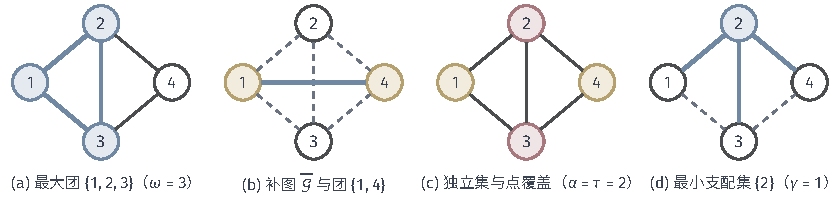
\includegraphics[width=129.000mm]{figures/03-graphs/01-structure-and-computation/tikz/graph-clique-indep-cover/figure.pdf}
  \caption{贯穿图上的团、补图、独立集、点覆盖与支配集。(a)蓝色顶点$\{1,2,3\}$两两相邻，构成最大团（$\omega(\mathcal G)=3$）；(b)补图$\overline{\mathcal G}$只含原图缺失的边$\{1,4\}$，原图的最大独立集$\{1,4\}$变成$\overline{\mathcal G}$的最大团；(c)黄色顶点$S=\{1,4\}$互不相邻，构成最大独立集（$\alpha(\mathcal G)=2$），其余红色顶点$V\setminus S=\{2,3\}$覆盖全部五条边，构成最小点覆盖（$\tau(\mathcal G)=2$）；(d)蓝色顶点$D=\{2\}$经三条蓝色粗边支配其余全部顶点$1,3,4$，构成最小支配集（$\gamma(\mathcal G)=1$），但虚线边$\{1,3\},\{3,4\}$未被它覆盖。}
  \label{fig:graph-clique-indep-cover}
\end{figure*}
